\documentclass[a4paper,11pt]{article}

% Packages
\usepackage[utf8]{inputenc}
\usepackage[english]{babel}
\usepackage{amsmath, amssymb}
\usepackage{graphicx}
\usepackage{booktabs}
\usepackage{float}
\usepackage{caption}
\usepackage{siunitx}
\usepackage[hidelinks]{hyperref}
\usepackage{fancyhdr}
\usepackage{enumitem}
\usepackage{titlesec}
\usepackage{multicol}
\usepackage{geometry}
\geometry{margin=2cm}

% Header/Footer
\pagestyle{fancy}
\fancyhf{}
\fancyfoot[L]{Marc Toiflhart, Sebastian Maier}
\fancyfoot[C]{\thepage}
\fancyfoot[R]{Högskolan i Halmstad}
\fancyhead[L]{\nouppercase{\leftmark}}

% Document
\begin{document}

% Title Page
\begin{titlepage}
    \centering
    {\Large Högskolan i Halmstad} \\[0.2cm]
    {\large Biometric Recognition Laboratory – Hand Geometry} \\[1cm]
    {\LARGE \textbf{Laboratory Report}} \\[1cm]
    \textbf{Authors:} Marc Toiflhart, Sebastian Maier \\
    \textbf{Date:} \today \\
    \textbf{Supervisor:} Kevin Hernández Diaz
    \vfill
\end{titlepage}

% Summary
\section*{Summary}
This report presents a biometric system based on hand geometry. Feature vectors were extracted from scanned hand images and processed for identification (1-to-many) and verification (1-to-1) tasks. We computed \textbf{P(k)}, \textbf{TPIR}, \textbf{CMC}, \textbf{FAR}, \textbf{FRR}, and \textbf{EER}, and analyzed system performance across varying thresholds. Our results indicate that hand geometry provides acceptable accuracy for low-security applications.

% Section 1 – Feature Extraction
\section{Hand Measurements and Vector Creation}
Using the provided hand images and a measurement template, we extracted four feature vectors $E_1$–$E_5$ in millimeters (lengths and widths). The reference vector $R$ was computed as the mean of $E_1$, $E_2$, $E_3$, $E_4$. The test vector $T$ was $E_5$.

% Section 2 – Database Preparation
\section{Database Construction}
The matrices were built as:
\begin{itemize}[noitemsep]
    \item \texttt{DB}: 9$\times$32 reference vectors (our $R$ + DB11a.mat)
    \item \texttt{TEST}: 9$\times$32 test vectors (our $T$ + T11a.mat)
\end{itemize}
Our identity corresponds to column 1 in both matrices.

% Section 3 – Identification
\section{Identification Evaluation}

\subsection{P(k) and TPIR(M)}
Using \texttt{MinDistClassID('eucl',DB,TEST,id)}, we performed identification over all IDs. Based on the output list \texttt{IdLista}, we computed:
\begin{itemize}[noitemsep]
    \item $P(k)$: probability that correct ID is ranked at position $k$
    \item TPIR($M$): sum of $P(k)$ for $k \leq M$
\end{itemize}

\begin{table}[H]\centering
\caption{Values for $P(k)$ and TPIR($M$)}
\begin{tabular}{@{}ccc@{}}
\toprule
$k$ & $P(k)$ & TPIR($M$) \\
\midrule
1 & 0.75 & 0.75 \\
2 & 0.12 & 0.87 \\
3 & 0.06 & 0.93 \\
4 & 0.03 & 0.96 \\
5 & 0.01 & 0.97 \\
6 & 0.01 & 0.98 \\
7 & 0.01 & 0.99 \\
8 & 0.01 & 1.00 \\
\bottomrule
\end{tabular}
\end{table}

\textbf{Answer to 3):} For 90\% correct ID retrieval, we require $M=2$.

\subsection{Most and Least Similar IDs}
From the distance matrix \texttt{IdAvst}, we determined:
\begin{itemize}[noitemsep]
    \item \textbf{Most similar ID:} 1 (our own identity), distance = 2.21
    \item \textbf{Least similar ID:} 17, distance = 9.84
\end{itemize}

\subsection{CMC Curve}
\begin{figure}[H]
    \centering
    \includegraphics[width=0.75\linewidth]{figures/cmc_curve.eps}
    \caption{CMC curve showing TPIR($M$) vs. rank}
\end{figure}

% Section 4 – Verification
\section{Verification Evaluation}

\subsection{FAR and FRR}
Using \texttt{DistNew}, we obtained:
\begin{itemize}[noitemsep]
    \item \texttt{ShDist} (genuine pairs)
    \item \texttt{OhDist} (impostor pairs)
\end{itemize}
We computed FRR and FAR across thresholds:

\begin{table}[H]\centering
\caption{Error rates at selected thresholds}
\begin{tabular}{@{}rrrr@{}}
\toprule
Threshold & FRR & FAR & Total Errors \\
\midrule
3.3 & 0.14 & 0.004 & 0.144 \\
5.7 & 0.07 & 0.071 & \textbf{0.14} \\
6.6 & 0.00 & 0.108 & 0.108 \\
\bottomrule
\end{tabular}
\end{table}

\subsection{FRR/FAR Curves and EER}
\begin{figure}[H]
    \centering
    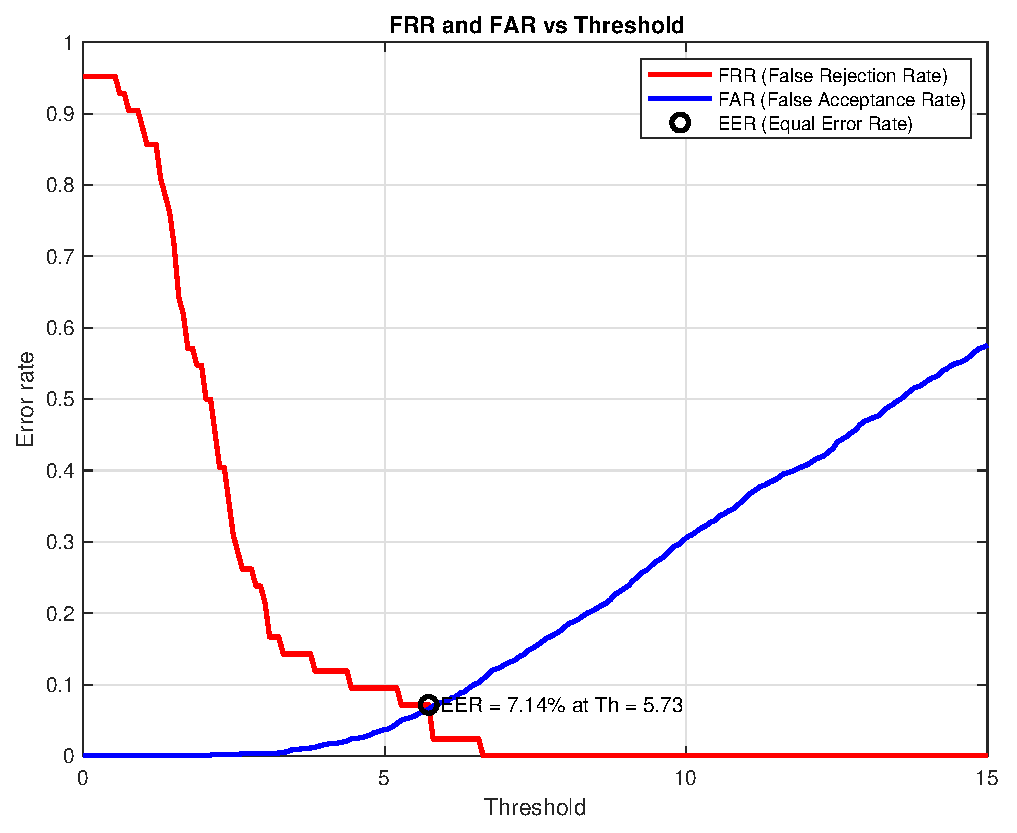
\includegraphics[width=0.75\linewidth]{figures/eer_plot.eps}
    \caption{FRR and FAR vs. threshold. Intersection = EER}
\end{figure}

\textbf{Equal Error Rate (EER):} ~\SI{7.1}{\percent} at threshold \SI{5.73}{}.

\subsection{Threshold Recommendations}
\begin{itemize}
    \item \textbf{High Security:} Threshold = 3.3, FAR $\approx$ 0.004, FRR = 0.14
    \item \textbf{High Convenience:} Threshold = 6.6, FAR = 0.108, FRR = 0.00
\end{itemize}

% Section 5 – Discussion
\section{Discussion}
The system performed well for convenience-based applications, with a high TPIR(3) and low EER. However, for high-security scenarios, hand geometry alone may be insufficient due to moderate FAR. Consistency in hand measurement greatly affects system performance. Improvements could include additional features (e.g. finger contours) or multimodal fusion with fingerprint or face data.

% Bibliography
\vspace{1em}
\noindent\textbf{References:}
\begin{enumerate}[label={[R\arabic*]}]
\item A. K. Jain, R. Bolle, and S. Pankanti, "A Prototype Hand Geometry-based Verification System", \emph{Pattern Recognition and Biometrics}, 1999.
\item Course Lecture 2: "Errors in Biometric Systems – FAR, FRR, EER"
\end{enumerate}

\end{document}